\Titular*%
{Pasatempos}%
{ Autoría múltiple}%
{pasatempos}%
{}%

\begin{refsection}
\vspace*{-6mm}
\section*{\textcolor{Resalte}{Encrucillado } {\normalfont \itshape Luis Arcas Morcillo}}%

% Descomentar para entrar no modo solución
% No modo solución todos os puzzles saen resoltos
% \PuzzleSolution
\begin{Puzzle}{27}{16}
|[1]P  |{}    |{}    |{}    |{}    |{}    |{}    |{}    |{}    |{}    |{}    |{}    |{}    |{}    |{}    |{}    |{}    |[2]P  |{}    |{}    |{}    |{}    |{}    |{}    |{}    |{}    |{}   |{} |.
|É     |{}    |{}    |{}    |{}    |{}    |{}    |{}    |{}    |{}    |{}    |{}    |{}    |{}    |{}    |{}    |{}    |O     |{}    |{}    |[3]C  |{}    |{}    |{}    |{}    |[4]F  |{}   |{} |.
|N     |{}    |{}    |[5]L  |U     |[6]Z  |{}    |{}    |{}    |{}    |{}    |{}    |{}    |{}    |{}    |{}    |{}    |[7]I  |N     |T     |E     |N     |S     |I     |D     |A     |D    |E  |.
|D     |{}    |{}    |{}    |{}    |E     |{}    |{}    |{}    |{}    |[8]C  |{}    |{}    |{}    |{}    |{}    |{}    |S     |{}    |{}    |R     |{}    |{}    |{}    |{}    |S     |{}   |{} |.
|U     |{}    |{}    |[9]É  |T     |E     |R     |{}    |{}    |[10]G |R     |I     |F     |[11]F |I     |T     |H     |S     |{}    |{}    |N     |{}    |{}    |{}    |{}    |E     |{}   |{} |.
|L     |{}    |{}    |{}    |{}    |M     |{}    |{}    |{}    |{}    |I     |{}    |{}    |Í     |{}    |{}    |{}    |O     |{}    |{}    |{}    |{}    |{}    |{}    |{}    |S     |{}   |{} |.
|[12]O |S     |[13]C |I     |L     |A     |D     |O     |R     |E     |S     |{}    |{}    |S     |{}    |{}    |{}    |[14]N |E     |W     |T     |O     |N     |{}    |{}    |{}    |{}   |{} |.
|{}    |{}    |U     |{}    |{}    |N     |{}    |{}    |{}    |{}    |T     |{}    |{}    |I     |{}    |{}    |{}    |{}    |{}    |{}    |{}    |{}    |{}    |{}    |{}    |{}    |{}   |{} |.
|{}    |{}    |A     |{}    |{}    |{}    |{}    |{}    |{}    |{}    |A     |{}    |{}    |C     |{}    |{}    |{}    |{}    |{}    |{}    |{}    |{}    |{}    |{}    |{}    |{}    |{}   |{} |.
|[15]V |E     |N     |U     |S     |{}    |{}    |{}    |[16]V |O     |L     |F     |R     |A     |[17]M |I     |O     |{}    |{}    |[18]C |{}    |{}    |{}    |{}    |{}    |{}    |{}   |{} |.
|{}    |{}    |T     |{}    |{}    |{}    |{}    |{}    |{}    |{}    |{}    |{}    |{}    |{}    |O     |{}    |{}    |{}    |{}    |A     |{}    |{}    |{}    |{}    |{}    |{}    |{}   |{} |.
|{}    |{}    |O     |{}    |{}    |{}    |{}    |{}    |{}    |{}    |{}    |{}    |{}    |[19]U |M     |A     |{}    |{}    |{}    |U     |{}    |{}    |{}    |{}    |{}    |{}    |{}   |{} |.
|{}    |{}    |{}    |{}    |{}    |{}    |{}    |{}    |{}    |{}    |{}    |{}    |{}    |{}    |E     |{}    |{}    |{}    |{}    |S     |{}    |{}    |{}    |{}    |{}    |{}    |{}   |{} |.
|{}    |{}    |{}    |{}    |{}    |{}    |{}    |{}    |{}    |{}    |{}    |{}    |{}    |[20]I |N     |E     |R     |C     |I     |A     |{}    |{}    |{}    |{}    |{}    |{}    |{}   |{} |.
|{}    |{}    |{}    |{}    |{}    |{}    |{}    |{}    |{}    |{}    |{}    |{}    |{}    |{}    |T     |{}    |{}    |{}    |{}    |{}    |{}    |{}    |{}    |{}    |{}    |{}    |{}   |{} |.
|{}    |{}    |{}    |{}    |{}    |{}    |{}    |{}    |{}    |{}    |{}    |{}    |{}    |{}    |O     |{}    |{}    |{}    |{}    |{}    |{}    |{}    |{}    |{}    |{}    |{}    |{}   |{} |.
\end{Puzzle}

% Como alternativa a este multicols, podería usarse varios minipages
\begin{multicols}{2}

\begin{PuzzleClues}{\textbf{Vertical}}\\
\Clue{1}{PÉNDULO}{O legado de Foucault na facultade}\\
\Clue{2}{POISSON}{Probablemente un peixe manchado}\\
\Clue{3}{CERN}{Centro de investigación europeo máis internacional}\\
\Clue{4}{FASES}{Son lunares ou diagramas}\\
\Clue{6}{ZEEMAN}{Ver dobre en cuántica débese a este efecto}\\
\Clue{8}{CRISTAL}{Disposición atómica ordenada}\\
\Clue{11}{FÍSICA}{Rama científica especializada no estudo da natureza e comportamento da materia, así como a forza e a enerxía}\\
\Clue{13}{CUANTO}{Canta enerxía?}\\
\Clue{17}{MOMENTO}{Teno esta revista}\\
\Clue{18}{CAUSA}{Precede ao efecto non relativista}\\
\end{PuzzleClues}

\begin{PuzzleClues}{\textbf{Horizontal}}\\
\Clue{5}{LUZ}{Onda e corpúsculo}\\
\Clue{7}{INTENSIDADE}{Voltaxe = ... $\times$ Resistencia}\\
\Clue{9}{ÉTER}{Se non se sabe o que é, posiblemente é isto}\\
\Clue{10}{GRIFFITHS}{O gran libro (polo menos en EM)}\\
\Clue{12}{OSCILADORES}{En esencia, todo son ... (pl.)}\\
\Clue{14}{NEWTON}{Físico nacido en Natividad}\\
\Clue{15}{VENUS}{Afrodisíaco planeta}\\
\Clue{16}{VOLFRAMIO}{Elemento W}\\
\Clue{19}{UMA}{Unidad de masa atómica}\\
\Clue{20}{INERCIA}{Principio de ..., o primeiro de tres}\\
\end{PuzzleClues}
\end{multicols}

%Causa • CERN • Cristal • Cuanto • Fases • Física • Griffiths • Inercia •
%Intensidade • Luz • Momento • Newton • Osciladores • Poisson • Péndulo • UMA •
%Venus • Volframio • Zeeman • Éter

\begin{center}
Solucións en orde alfabético, ofuscadas co cifrado ROT13 (buscade en internet \texttt{rot13 decode} para ver as solucións):

\vspace*{1em}

PNHFN PREA PEVFGNY PHNAGB SNFRF SÍFVPN TEVSSVGUF VAREPVN VAGRAFVQNQR YHM
ZBZRAGB ARJGBA BFPVYNQBERF CBVFFBA CÉAQHYB HZN IRAHF IBYSENZVB MRRZNA ÉGRE
\end{center}

\section*{\textcolor{Resalte}{Exercicios para relaxarnos}  {\normalfont \itshape Álvaro Pallas Otero}   \hfill     {\small (Fonte: @Ankxparch en Instagram)}}%

\begin{multicols}{2}
\begin{gather*}
    \text{i)} \sum_{k=0}^\infty \frac{4(-1)^k}{2k+1}
\end{gather*}\\
\begin{gather*}
    \text{ii)} \lim_{n\rightarrow \infty} n\left(\int_0^1 \sqrt[n]{x^2+1}\text{d}x -1\right)
\end{gather*}
\end{multicols}

\newpage

\section*{\textcolor{Resalte}{Colgando cadros} {\normalfont \itshape Víctor Díaz Díaz}}%

\begin{multicols}{2}

Queremos colgar un cadro dunha parede empregando $n$ cravos, de xeito que
quitando \textbf{un único cravo calquera} o cadro caia polo seu peso, ignorando
fricción.\\
Para o caso $n=1$ (caso trivial), a solución sería a mostrada figura contigua \ref{fig:solucion_victor}. O problema consiste en encontrar unha solución para polo menos $n=3$ gráfica o/e analítica. Tamén, pódese construír unha solución xeral analítica (non única) para un $n$ arbitrario recorrendo á teoría de grupos.

\nocite{Demaine_2013}
\printbibliography
\hfill
\goodbreak

\begin{center}
    \captionsetup{justification=centering}
    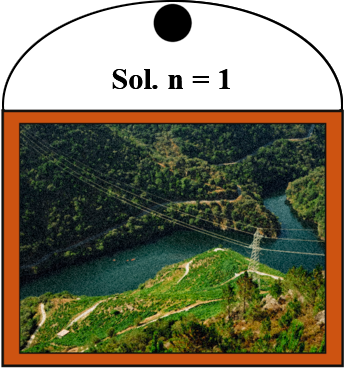
\includegraphics[width=0.7\linewidth]{revistas/002/imaxes/solucion_victor.png}
    \captionof{figure}{Solución para $n=1$}
    \label{fig:solucion_victor}
\end{center}

\end{multicols}
\end{refsection}
% Ola son Adrián vou copypastear o meu. Grazas Adrian, amamoste
% Dubidoo moito, entreguei mais tarde imposible. Shhh, non negues o noso amor por ti
% si gracioso é un rato ajsajja
% Si si acabome de dar de conta pero éme máis gracioso isto 
%jjjjjjj
% QUE NADIE BORRE ESTO, QUE QUEDE PARA A POSTERIDADE !!
% POR FAVOR PEDÍMLO TODOS 
\section*{\textcolor{Resalte}{Física ou Fortuna \#1: Vaime chover na praia?} {\normalfont \itshape Adrián Vázquez Velasco}}%

\begin{multicols}{2}

Iniciamos neste número unha sección recurrente de desafíos físicos: ``Física ou Fortuna''. O obxectivo será intentar estimar un problema que non ten unha resposta obvia. Cun formulario online, recolleranse as respostas daqueles que queiran participar. Animamos a todos os lectores a cubrir o formulario e pasar un bo rato esforzándose para as respostas tanto (ou tan pouco) como vexan oportuno. En base aos resultados, elaborarase unha clasificación á que se irán engadindo as cuestións dos seguintes números.

\begin{center}
    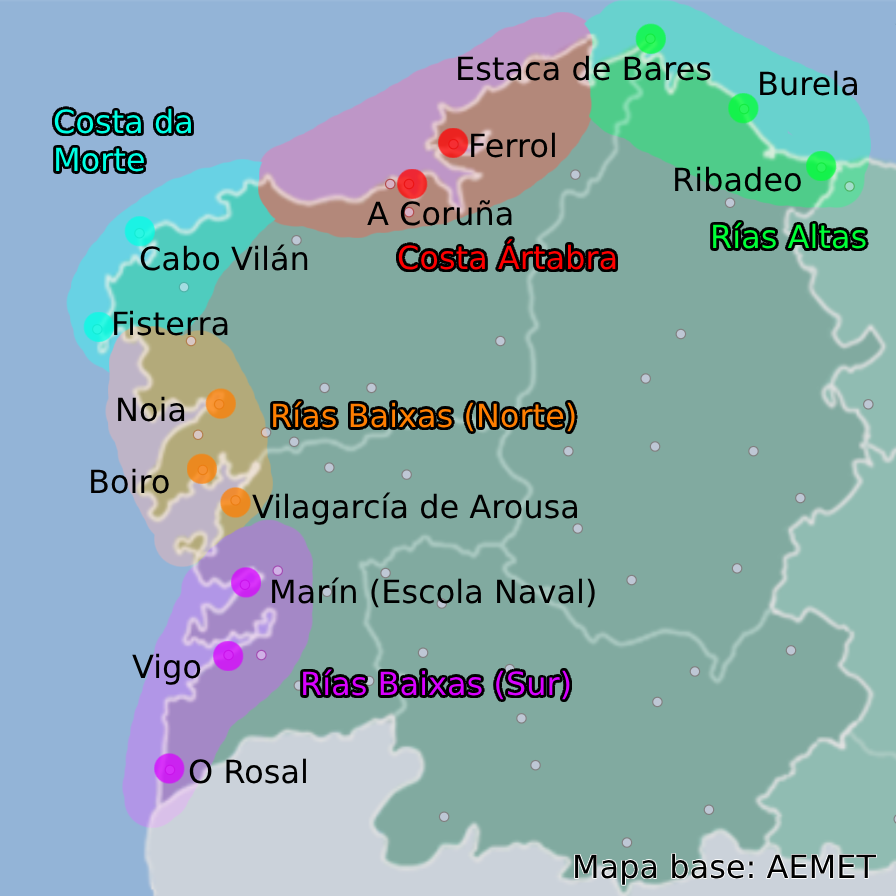
\includegraphics[width=0.8\linewidth]{revistas/002/imaxes/mapa.png}
\end{center}

Nesta edición, queremos propórvos como reto unha serie de cuestións sobre a choiva na costa este verán. Para iso, tomaranse os datos da AEMET \textbf{dende o 1 de xullo ata o 31 de agosto deste ano} (62 días en total), en 13 estacións meteoroloxicas da costa galega, escollidas por seren facilmente accesibles en tempo real na súa web. En concreto, as do mapa da esquerda.
%\begin{enumerate} %isto probablemente métolle tixeretazo limpo
%	\item \textit{Rías Altas/A Mariña}: Ribadeo, Burela, Estaca de Bares.
%	\item \textit{Costa Ártabra}: Ferrol, A Coruña.
%	\item \textit{Costa da Morte}: Cabo Vilán, Fisterra.
%	\item \textit{Rías Baixas (Norte)}: Noia, Boiro, Vilagarcía de Arousa.
%	\item \textit{Rías Baixas (Sur)}: Escola Naval de Marín, Vigo, O Rosal.
%\end{enumerate}

\vspace{4px}
As cuestións a intentar predecir son as seguintes:
\vspace{-4px}
\begin{enumerate}
	\item Cal será a \textit{precipitación acumulada en mm de auga} (con resolución de 0.1 mm) recollida en \textbf{promedio entre todas as estacións} nos 62 días? É dicir, a media dos respectivos totais de precipitación.
	\item Elabora unha \textit{orde de maior a menor precipitación acumulada} entre os promedios das \textbf{5 zonas costeiras} especificadas.
	\item Cal será o \textit{número mínimo de días con precipitacións} entre as \textbf{13 estacións} e en cal delas se dará? Cal será o \textit{número máximo de días con precipitacións} entre as \textbf{13 estacións} e en cal se dará?
\end{enumerate}
 
O formulario é accesible a traves do Linktree e pecharase o \textbf{domingo 15 de xuño ás 23:59} coa fin de evitar ter en conta predicións meteorolóxicas concretas, pero deixando moita marxe por estar en época de exames.

\begin{center}
    
\includegraphics[width=0.4\linewidth]{revistas/002/imaxes/pasatempos_momentum.png}
    \url{https://linktr.ee/pasatempos.momentum}
\end{center}

\end{multicols}